\section{Evaluation}
\label{sec:evaluation}

\subsection{Experiments}

All tests are conducted on a desktop Intel i5 4-Core @ 3.2GHz. A TTree with 100 million float values is read with different APIs. We tested three different use cases: GetBulkEntries, TTreeReaderFast and RDataSource.

\subsection{Results}

Figure \ref{fig:tbranch} shows the time spent on iterating all events in the \textit{TTree} with \textit{GetEntry} and \textit{GetBulkEntries}. Figure \ref{fig:ttreereader} shows the read time between \textit{TTreeReader} and \textit{TTreeReaderFast}. As shown in the figures, Bulk IO spends 10+ times less than \textit{GetEntry} and \textit{TTreeReader}. Bulk IO in both use cases spends similar time on reading events. \textit{TTreeReader} interface spends more than 3 times reading events than \textit{GetEntry} due to the overheads of TTreeReader itself (TTreeReader internally calls \textit{GetEntry}). 

\begin{figure}[!ht]
\centering
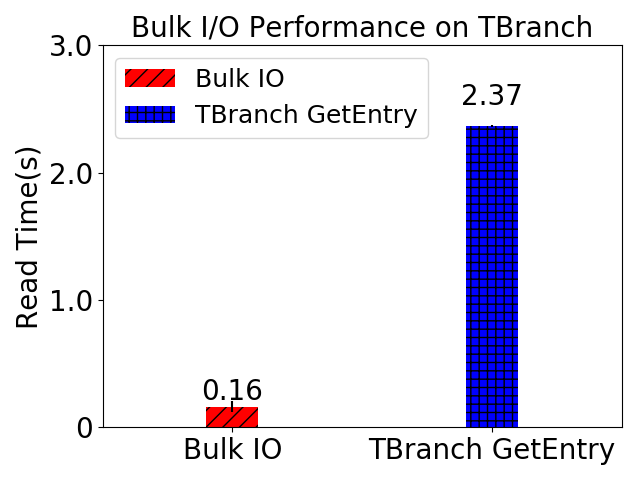
\includegraphics[height=2.5in, width=3.5in]{getbulkentries.png}
\vspace*{-2mm}
\caption{Performance between \textit{GetEntry} and \textit{GetBulkEntries}.}
\label{fig:tbranch}
\end{figure}

\begin{figure}[!ht]
\centering
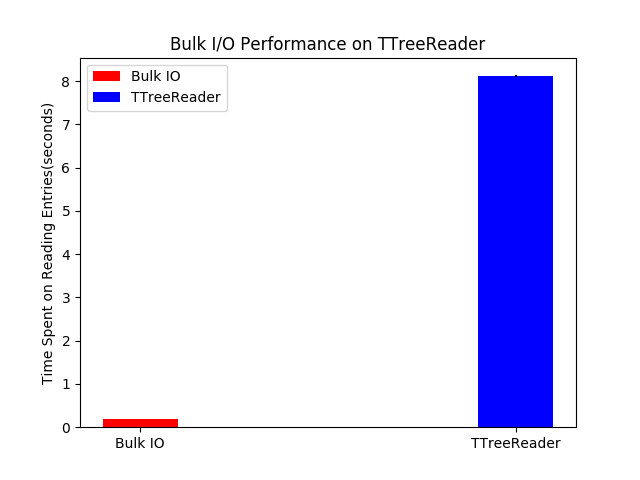
\includegraphics[height=2.5in, width=3.5in]{ttreereader.png}
\vspace*{-2mm}
\caption{Performance between \textit{TTreeReader} and \textit{TTreeReaderFast}.}
\label{fig:ttreereader}
\end{figure}

\begin{figure}[!ht]
\centering
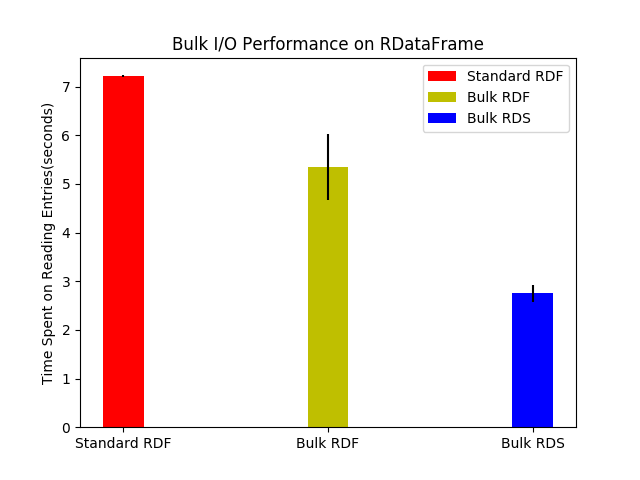
\includegraphics[height=2.5in, width=3.5in]{dataframe.png}
\vspace*{-2mm}
\caption{Performance improvements on RDataFrame with Bulk IO.}
\label{fig:rdataframe}
\end{figure}

Figure \ref{fig:rdataframe} shows the results of Bulk IO in RDataFrame. In the figure, the standard RDF shows the performance by using regular RDataFrame function calls. Bulk RDF and Bulk RDS show the result of Bulk APIs. The difference is that, Bulk RDS test detaches RDataSource from RDataFrame stack and run the test directly through RDS function calls. As shown in Figure \ref{fig:rdataframe}, Bulk RDS outperforms standard RDF by more than 2 times. In addition, RDataFrame has extra overheads compared to RDataSource (RDataFrame internally relies RDataSource), therefore Bulk RDF runs slower than Bulk RDS, but still outperforms standard RDF.
